% if you want to print your thesis on one side on the papar, use 'oneside' option 
% if you want to print your thesis on both sides on the papr, do not use 'oneside' option
% the template will generate blank pages bwteen title pages, sections, list of contents ...
\documentclass[11pt,b5paper,oneside]{snuthesis-kor}
%\documentclass[11pt,b5paper]{snuthesis-kor}
%\special{papersize=8.5in,11in}

%%%%%%%%%%%%%%%%%%%%%%%%%%%%%%%%%%%%%%%%%%%%%%%
% include additional packages you need to use
%%%%%%%%%%%%%%%%%%%%%%%%%%%%%%%%%%%%%%%%%%%%%%%
% graphic, float package
\usepackage{graphicx}		% for setting images
\usepackage{float}			% for float objects
\usepackage{subfigure}		% for adding several figures in a figure environment
\usepackage{lscape}			% for landscape type images or tables
\usepackage{url}

% mathmetical presentation
\usepackage{gensymb}
\usepackage{amsmath}
\usepackage{amsfonts}
\usepackage{amssymb}
\usepackage{amsthm}
%\usepackage{mathptm}
\usepackage{exscale}
\usepackage{textcomp}		% extra symbols
\usepackage{comment}
\usepackage{upgreek}
\usepackage{bigstrut}
\usepackage{stfloats}
\usepackage{color}
\usepackage{here}
\usepackage[mathcal]{eucal}
\DeclareSymbolFont{usualmathcal}{OMS}{cmsy}{m}{n}
\DeclareSymbolFontAlphabet{\mathcal}{usualmathcal}

% package for using algorithmic presentation
\usepackage{algorithmic}
\usepackage{algorithm}
% customize algorithmic environment
\renewcommand{\algorithmicrequire}{\makebox[40px]{\hfill\textbf{Input :}}}
\renewcommand{\algorithmicensure}{\makebox[40px]{\hfill\textbf{Output :}}}


% array and table presentation
\usepackage[utf8]{inputenc} 
\usepackage{array}
\usepackage{multirow}
\usepackage[table]{xcolor}
%\usepackage{ctable}
\usepackage{booktabs}		% for typesetting tables at the level of publication		
							% do not use vertical rule


%%%%%%%%%%%%%%%%%%%%%%%%%%%%%%%%%%%%%%%%%%%%%%%
% set document layout and default look and feel such spacings and indentations
%%%%%%%%%%%%%%%%%%%%%%%%%%%%%%%%%%%%%%%%%%%%%%%

% set page layout, default margin is 3cm
\geometry{margin=3cm}

% set double spacing
\doublespacing

% set indentation
\setlength{\parindent}{2em}

% if you do not want indent first paragraph in each chapter, section, and sub sections
% remove below line
%\usepackage{indentfirst}

% if you want to make vertical spaces between paragraphs,
% removfe comments the below line and change dime '10pt' as what you want 
\setlength{\parskip}{10pt}

% adjust spacing below the caption 
\setlength{\belowcaptionskip}{5pt}


% if you want to make index, 
% use \makeindex in preamble, 
% use \index at the word you want to index, 
% and use \printindex where you want to print the index
\makeindex


% hyperref package can generate pdf references
% must be loaded at last
%\usepackage[unicode]{hyperref}


% define new theorem like entities you need
\newtheorem{lemma}{Lemma}
\newtheorem{definition}{Definition}

%%%%%%%%%%%%%%%%%%%%%%%%%%%%%%%%%%%%%%%%%%%%%%%
% set parper variables
% thesis summary
%\title{낸드 플래시 기반 저장장치\\ 성능 및 수명 개선 기법} 

\title{{\LARGE 낸드 플래시 저장장치 수명 향상을 위한 응용프로그램 특성 기반 계층 교차 최적화 기법}}
\engtitle{{\Large Cross-Layer Optimization Techniques for Extending Lifetime of NAND Flash-Based Storage Devices
Exploiting the Application Characteristics}}
%\keywords{NAND Flash Memory, Flash-Based Storage Devices, Storage Performance Optimization, Operating System, Embedded System, Storage Reliability Management}
\keywords{NAND Flash Memory, NAND Flash-Based Storage Devices, Storage Lifetime, Embedded Software}
\engkeywords{낸드 플래시 메모리, 플래시 기반 저장 장치, 저장장치 수명, 임베디드 소프트웨어}


\university{서울대학교 대학원}
\enguniversity{The Graduate School\\Seoul National University}
\collegeordept{전기$\cdot$컴퓨터 공학부}
\engcollegeordept{Department of Electrical Engineering & Computer Science}

\author{김태진}
\engauthor{Taejin Kim}
\studentnumber{2012-30201}
\hpnumber{010-8817-0050}

% degree 
\msorphd{공학박사}
\degreetitle{공학박사}

% dates
\submitdate{}
\acceptdate{}
\degreedate{}
\agreedate{}


% advisor and commitees
% If you are writing master thesis, just do not fill commiteeb and commiteec, 
% then agreement page will be automatically adjusted. 
\advisor{지도교수~~~~김~지~홍}
\chief{~~~~~~~~~~~~~~~~~~~~~~~~~~~}
\vicechief{~~~~~~~~~~~~~~~~~~~~~~~~~~~}
\commiteea{~~~~~~~~~~~~~~~~~~~~~~~~~~~}
\commiteeb{~~~~~~~~~~~~~~~~~~~~~~~~~~~}
\commiteec{~~~~~~~~~~~~~~~~~~~~~~~~~~~}
%%%%%%%%%%%%%%%%%%%%%%%%%%%%%%%%%%%%%%%%%%%%%%


%%%%%%%%%%%%%%%%%%%%%%%%%%%%%%%%%%%%%%%%%%%%%%%
% start thesis
%%%%%%%%%%%%%%%%%%%%%%%%%%%%%%%%%%%%%%%%%%%%%%%
\begin{document}


% set page style as not generating page numbers
\pagestyle{empty}

%title page
\maketitle

%submission page
\makesubmission

%%agreement page
%\makeagreement

% set page style as generating roman page numbers
\newpage
\pagestyle{plain}
\pagenumbering{roman}
\setcounter{page}{1}


\begin{abstract}

Replacing HDDs with NAND flash-based storage devices (SSDs) has been one of the major 
challenges in modern computing systems especially in regards to better performance and higher mobility.
Although the continuous semiconductor process scaling and multi-leveling techniques 
lower the price of SSDs to the comparable level of HDDs, the decreasing lifetime of NAND flash memory, 
as a side effect of recent advanced device technologies, 
is emerging as one of the major barriers to the wide adoption of SSDs in high-performance computing systems.

In this dissertation, system-level lifetime improvement techniques for
recent high-density NAND flash memory are proposed.
Unlike existing techniques, the proposed techniques resolve the
problems of decreasing lifetime by exploiting the write request characteristics,
such as context of I/O or duplicate data contents.

We first propose a system-level approach to reduce WAF that exploits
the I/O context of an application to increase the data lifetime prediction
for the multi-streamed SSDs. 
Since the key motivation behind the proposed technqiue was 
that data lifetimes should be estimated at a higher abstraction level than LBAs, 
we employ a write program context as a stream management unit.
Thus, it can effectively separate data with
short lifetimes from data with long lifetimes to improve the efficiency of garbage collection.

Second, we present a write traffic reduction approach which reduces the amount of
write traffic sent to a storage by eliminating redundant data, therby improving
the lifetime of storage devices. 
In particular, we improve the likelihood of eliminating redundant data
by introducing sub-page chunk based on the understanding of duplicate contents
such as partial updates or zero padding of file system.
It also resolves technical difficulties caused by its finer granularity, i.e., increased memory requirement and read
response time. 

In order to evaluate the effectiveness of the proposed techniques, we performed 
a series of evaluations using both a trace-driven simulator and emulator with I/O
traces which were collected from various real-world systems.
To understand the feasibility of the proposed techniques, we also implemented them
in Linux kernel on top of our in-house flash storage prototype and then evaluated
their effects on the lifetime while running real-world applications.
Our experimental results show that system-level optimization techniques are
more effective over existing optimization techniques.

\end{abstract}


%========================================================================
% table of contents, list of figures and tables
% rename toc, lof, lot, and ref
\renewcommand{\contentsname}{Contents}
\renewcommand{\listfigurename}{List of Figures}
\renewcommand{\listtablename}{List of Tables}
\renewcommand{\bibname}{Bibliography}


%========================================================================
\tableofcontents

\listoffigures
 
\listoftables


%========================================================================
% set page style as generating arabic page numbers
\clearpagebefore
\pagenumbering{arabic}
\setcounter{page}{1}

%========================================================================
% main body

\chapter{Introduction} 
\label{chap:Introduction}

\section{Motivation}
\label{sec:Intro_Motivation}

NAND flash-based solid-state drives (SSDs) are widely used in personal computing systems as well as mobile embedded systems.
However, in enterprise environments, SSDs are employed in only limited applications because SSDs are not yet cost competitive with HDDs~\cite{Janus_albrecht}.
Fortunately, the prices for SSDs have fallen to the comparable level of HDDs by continuous semiconductor process scaling (e.g., 10 nm-node process~\cite{15nmMLC_Sako}) combined with multi-leveling technologies (e.g., MLC~\cite{21nmMLC_Kim} and TLC~\cite{TLC_Shin}).
However, the limited endurance of NAND flash memory, which have declined further as a side effect of the recent advanced device technologies, is emerging as another major barrier to the wide adoption of SSDs.
(\textit{NAND endurance} is the ability of a memory cell to endure program/erase (P/E) cycling, and is quantified as \textit{the maximum number $N_{P/E}^{max}$ of P/E cycles} that the cell can tolerate while maintaining its reliability requirements~\cite{Flash_Brewer}.)
For example, although the NAND capacity per die doubles every two years, the actual lifetime (which is proportional to the total NAND capacity and $N_{P/E}^{max}$) of SSDs does not increase as much as projected in the past seven years because $N_{P/E}^{max}$ have declined by 70\% during that period~\cite{MooresLaw_chien}.
In order for SSDs to be commonplace in enterprise environments, the issues concerning NAND endurance should be properly resolved.

Since the Lifetime $L_{C}$ of an SSD with the total capacity $C$ is proportional to the maximum number $N_{P/E}^{max}$ of P/E cycles, and is inversely proportional to the total written data $W_{day}$ per day, $L_{C}$ (in days) can be expressed as follows (assuming a perfect wear leveling):
\begin{equation}\label{eq:introduction_1}
L_{C} = \frac{N_{P/E}^{max}\: \times \: C}{W_{day}\: \times \: WAF} \quad ,
\end{equation}
where $WAF$ is a write amplification factor which represents the efficiency of an FTL algorithm.
Many existing lifetime-enhancing techniques have mainly focused on reducing $WAF$ by increasing the efficiency of an FTL algorithm.
For example, by avoiding unnecessary data copies during garbage collection, $WAF$ can be reduced~\cite{HotCold_Hsieh}.
In order to reduce $W_{day}$, various system-level techniques were proposed.
For example, data de-duplication~\cite{CAFTL_Chen}, data compression~\cite{Compression_Lee}, and write traffic throttling~\cite{DT_Lee} are such techniques.
On the other hand, only a few system/software-level techniques have been proposed to increase $N_{P/E}^{max}$.
Although several conceptual device-level techniques (e.g., a self-healing SSD~\cite{SelfHealing_Wu}) were suggested regarding $N_{P/E}^{max}$, it is difficult for these to be employed in real systems because of their unrealistic hardware settings and critical side-effects.

By exploiting the tradeoff relationships between the NAND characteristics (e.g., capacity, performance, retention, and endurance), several cross-layer optimization techniques have been suggested.
In order to improve SSD performance, for example, the retention relaxation technique~\cite{RetentionRelaxation_Liu} temporarily relaxes the NAND retention capability while FlexFS~\cite{Flexfs_Lee} flexibly reorganizes the NAND capacity between SLC and MLC regions.
Although these techniques exploited the device-level physical characteristics in the similar fashion of our work, their main goals are quite different from ours.
Up until now, there have been a few particular suggestions to improve the NAND endurance by exploiting the tradeoff relationships between the NAND capabilities.


\section{Dissertation Goals}
\label{sec:Intro_ResearchGoals}

In this dissertation, we propose new cross-layer optimization techniques to extend the lifetime of NAND flash-based storage devices by exploiting the tradeoff relationship among NAND capabilities such as endurance, performance, and retention.
%Our proposed techniques enables a system software to directly exploit the tradeoff relationship between the NAND endurance and NAND operating voltages/times so that the NAND requirements, such and endurance, performance, and retention, can be properly managed.
The primary goals of this dissertation is as follows:

\begin{itemize}
\item Enabling a system software to exploit the tradeoff relationship between the endurance and the other capabilities of NAND flash memory.
\item Developing system-level techniques to improve NAND endurance while maintaining the other NAND requirements.
\item Providing reliability preservation techniques for NAND flash-based storage systems when flash-optimization techniques are widely employed in real environments.
\end{itemize}


\section{Contributions}
\label{sec:Intro_Contributions}

The proposed cross-layer approach in this dissertation adds a new dimension to the decreasing lifetime problem of NAND flash-based storage devices as follows:

\begin{itemize}
\item {\bfseries A unified NAND endurance model} which captures the tradeoff relationship between NAND endurance and the performance/retention capabilities of NAND flash memory is proposed.
We reveal that endurance degradation is primarily caused by excessive erase operations, and suggest effective device-level means (i.e., various write-capability tuning techniques) of alleviating the negative impact of erase operations on NAND endurance.
Based on the proposed NAND endurance model, a system software can adjust the internal operation voltages and times of NAND flash memory in a reliable fashion.
\item {\bfseries System-level lifetime improvement techniques} for NAND flash-based storage devices are presented.
Based on the NAND endurance model, the proposed techniques dynamically change the NAND performance and retention capabilities for each program operation so that endurance-enhancing erase operations can be frequently used.
Since the proposed lifetime improvement techniques can efficiently adapt to varying characteristics of I/O workload by accurately predicting the write performance and retention requirements, the overall performance and reliability requirements of storage systems are maintained while significantly improving NAND endurance.
%select the erase scaling modes and write tuning modes depending on varying workload conditions.
\item {\bfseries Reliability management techniques} for NAND flash-based storage systems are suggested.
Since the proposed lifetime improvement techniques aggressively tune down the NAND retention capability to improve NAND endurance, the retention-failure problem can be a serious technical issue for power/temperature-unstable computing environments.
In order to preserve the data durability of the stored data in NAND flash memory, we introduce a novel data recovery technique which can efficiently and quickly recover corrupted data from retention failures.
\end{itemize}

Although this dissertation has mainly focused on improving NAND endurance, our proposed techniques can be extended to improve other requirements (e.g., performance, retention, and read-disturbs resistance) of storage systems.
Moreover, since our techniques are entirely independent on data content, the existing flash-optimization techniques can be easily integrated into our proposed framework.


\section{Dissertation Structure}
\label{sec:Intro_DissertationStructure}


%The rest of the paper is organized as follows.
%Before our proposed techniques are presented, we briefly review the design principle of NAND flash memory in Section~\ref{sec:Background} and the previously proposed lifetime-enhancing techniques in Section~\ref{sec:RelatedWorks}.
%Section~\ref{sec:DynamicEraseVoltageTimeScaling} describes the proposed erase voltage and time scaling technique.
%In Section~\ref{sec:DynamicWriteModeTuning}, the dynamic write-tuning techniques and the NAND endurance model are presented.
%Our autoFTL with dynamic write-speed tuning modes is proposed in Sections~\ref{sec:autoFTL}, and experimental results follow in Section~\ref{sec:ExperimentalResults}.
%Section~\ref{sec:autoFTLplus.tex} explains our ongoing works for designing autoFTL$^{+}$ with dynamic retention tuning and its initial experimental results.
%Finally, Section~\ref{sec:Conclusion} concludes with a summary and future work.

This dissertation consists of seven chapters.
The first chapter presents a introduction to this dissertation while the last chapter serves as a conclusion with a summary and future work.
The five intermediate chapters are organized as follows:

Chapter~\ref{chap:Background} reviews the operational principles of NAND flash memory and explains existing SSD lifetime improvement techniques closely related to this dissertation.

Chapter~\ref{chap:DynamicEraseVoltageTimeScaling} describes the dynamic NAND voltage and time scaling framework which includes erase voltage/time scaling and write capability tuning.
Combining erase scaling and write tuning, a unified NAND endurance model for estimating their effects on NAND endurance is also suggested.

Chapter~\ref{chap:LifetimeImprovementWPT} proposes an SSD lifetime improvement technique using write-performance tuning.
%We explain how to select appropriate erase and write modes and show how much NAND endurance is improved.
We explain how to use a lower voltage and a slower speed for an erase operation and how to write data to a NAND block erased with a lower voltage.
In addition, the effect of the proposed technique on NAND endurance is presented in detail.

Chapter~\ref{chap:LifetimeImprovementRCT} presents a comprehensive SSD lifetime improvement technique using both write-performance tuning and retention-capability tuning.
We describe reliable prediction schemes to accurately predict the write performance and retention requirement and present efficient adaptation schemes to manage the NAND capabilities.
We then show how much NAND endurance is improved and whether the overall NAND requirements are preserved.

Chapter~\ref{chap:ReliabilityPreservationTechnique} suggests a reliability management technique in order to recover data loss due to retention failures.
Finally, we show how efficient the proposed technique is in terms of data recovery power and speed.



\chapter{Background} 
\label{chap:Background}


In order to improve NAND endurance, reliability and performance parameters are dynamically changed during run time in this dissertation.
In this chapter, we review the basics of key \textit{Vth} design parameters and the principals of a NAND program operation.


\section{Threshold Voltage Window of NAND Flash Memory}
\label{sec:Background_ThresholdVoltageWindow}

NAND flash memory stores data into cells by changing their \textit{Vth} states depending on bit information, and restores data from cells by sensing their \textit{Vth} states.
Figure~\ref{fig:Background_VthDistribution} illustrates an example of \textit{Vth} distributions for an MLC NAND device which stores two bits in a cell by using four distinct \textit{Vth} states distinguished by three read reference voltages.


\begin{figure}[t]
\centering
%\includegraphics[scale=1.15]{./Figures/2_Background/VthDistribution.eps}
\caption{An example of \textit{Vth} distributions for MLC NAND flash memory and primary \textit{Vth} design parameters for the NAND requirements.}
\label{fig:Background_VthDistribution}
\end{figure}


Aside from serving as a non-volatile storage medium, MLC NAND devices are also required to meet the specified NAND requirements~\cite{Flash_Brewer}.
For example, read and program operations of an MLC device should be completed within 100 $\mu$s and 1,600 $\mu$s, respectively~\cite{MooresLaw_chien}.
Moreover, even after 3,000 P/E cycles, it is required to support up to 400,000 read operations~\cite{MooresLaw_chien} as well as to retain its stored data for up to 1 year at $30\,^{\circ}\mathrm{C}$~\cite{Cox_JEDEC}.
Since the \textit{Vth} design parameters shown in Figure~\ref{fig:Background_VthDistribution} are closely related to the NAND requirements, the overall \textit{Vth} distributions should be carefully designed to meet all the NAND requirements under the worst-case operating conditions for a storage product.


The upper \textit{Vth} target {\small $V^{Erase}_{Verify}$} of the $E$ state is one of the key factors in determining the total width {\small$W_{Vth}$} of \textit{Vth} distributions.
As {\small $V^{Erase}_{Verify}$} is lowered, {\small $W_{Vth}$} gets widened so that it is easier to optimize the \textit{Vth} parameters for higher performance or longer retention capability.
However, as a side-effect of the lowered {\small $V^{Erase}_{Verify}$}, NAND endurance may deteriorate because NAND blocks are more deeply erased~\cite{DPES_jeong}.
Conversely, when a higher {\small $V^{Erase}_{Verify}$} is used, designing \textit{Vth} distributions becomes more complex because less {\small $W_{Vth}$} is available.


The width {\small $W_{Pi}$} of a \textit{Vth} distribution is mostly determined by the NAND write performance requirement.
Since NAND flash memory generally uses the incremental step pulse programming (ISPP) scheme to form \textit{Vth} distributions, {\small $W_{Pi}$} and the program time are directly affected by the ISPP step control.
For example, when a fine-grained ISPP step control is used for a program operation, {\small $W_{Pi}$} can be shortened while the program time increases~\cite{DPES_jeong}.
As a result, {\small $W_{Pi}$} is determined by the minimum achievable width of a \textit{Vth} distribution under the given program-time requirement.


The \textit{Vth} gap {\small $M_{Pi}$} between two adjacent states is mainly determined by the NAND retention requirement.
When NAND memory cells are programmed and left for a long time, charge loss may occur because stress-induced damage in the tunnel oxide layer is likely to loosen stored charges.
Since this charge-loss phenomenon may cause \textit{Vth} changes, it is necessary for a sufficient {\small $M_{Pi}$} to tolerate the \textit{Vth} changes.
In order to guarantee the NAND retention requirement under the worst-case operating condition, {\small $M_{Pi}$} is determined by the maximum \textit{Vth} change after the maximum number of P/E cycles and the specified retention time.


The \textit{Vth} gap {\small $M_{Dist}$} between the $E$ state and {\small $V_{Read}^{P1}$} primarily affects the program-disturbance resistance and read-disturbance resistance of NAND flash memory.
When NAND memory cells are programmed or read, neighbor cells that belong to the $E$ state may be softly programmed so that their \textit{Vth}s move to the right~\cite{Flash_Brewer}\cite{BER_mielke}.
In order to compensate for the \textit{Vth} changes due to these disturbances, a sufficient {\small $M_{Dist}$} should be reserved in the \textit{Vth} window as shown in Figure~\ref{fig:Background_VthDistribution}.
Typically, {\small $M_{Dist}$} is decided by the \textit{Vth} changes after the maximum number of P/E cycles followed by the maximum number of read cycles.


The read pass voltage {\small $V^{Pass}_{Read}$} which affects the NAND read disturbance is another key factor in deciding the value of {\small $W_{Vth}$}.
Since the NAND read disturbance has an exponential dependence on the {\small$V^{Pass}_{Read}$}~\cite{ReadDisturb_Kang}, {\small $V^{Pass}_{Read}$} is usually fixed as low as possible in device design times.
The \textit{Vth} gap {\small $M_{Pass}$} between the $P3$ state and {\small$V^{Pass}_{Read}$} is also essential to fully turn on all the NAND memory cells in a block~\cite{Flash_Brewer}.


When the \textit{Vth} design parameters are designated accordingly, all the \textit{Vth} states are placed between {\small $V^{Erase}_{Verify}$} and {\small $V^{Pass}_{Read}$}.
Therefore, the total width {\small $W_{Vth}$} of the \textit{Vth} window is expressed as follows (for an MLC NAND device):
\begin{equation}\label{eq:Background_Wvth}
\begin{split}
W_{Vth} &= V^{Pass}_{Read} - V^{Erase}_{Verify} \\
        &= M_{Dist} + \sum_{i=1}^{3} W_{Pi} + \sum_{i=1}^{3} M_{Pi} + M_{Read} .
\end{split}
\end{equation}
Since the \textit{Vth} design parameters are highly related to one another, if a certain design parameter is to be changed, we should check its effect on the whole \textit{Vth} window.


\section{NAND Program Operation}
\label{sec:Background_NANDProgramOperation}

In order to form a threshold voltage distribution within a desired region, NAND flash memory generally uses the incremental step pulse programming (ISPP) scheme.
As shown in Figure~\ref{fig:Background_ISPP}, the ISPP scheme gradually increases the program voltage by the $V_{ISPP}$ step until all the memory cells in a page are located in a desired threshold voltage region.
While repeating ISPP loops, once NAND cells are verified to have been sufficiently programmed, those cells are excluded from subsequent ISPP loops.


\begin{figure}[!t]
\centering
%\includegraphics[scale=1.1]{./Figures/2_Background/ISPP_Operation.eps}
\caption{A conceptual timing diagram of the ISPP scheme.}
\label{fig:Background_ISPP}
\end{figure}


Since the program time is proportional to the number of ISPP loops (which are inversely proportional to $V_{ISPP}$), the program time $T_{PROG}$ can be expressed as follows:
\begin{equation}\label{eq:Background_Tpgm}
T_{PROG} \propto \frac{V_{PGM}^{end} - V_{PGM}^{start}}{V_{ISPP}}.
\end{equation}


Figure~\ref{fig:Background_TprogVispp} shows normalized $T_{PROG}$ variations over different $V_{ISPP}$ scaling ratios. (When a $V_{ISPP}$ scaling ratio is set to $x$\%, $V_{ISPP}$ is reduced by $x$\% of the nominal $V_{ISPP}$.)
When a narrow threshold voltage distribution is needed, $V_{ISPP}$ should be reduced for a fine-grained control, thus increasing the program time.
Since the width of a threshold voltage distribution is proportional to $V_{ISPP}$~\cite{ISPP_suh}, for example, if the nominal $V_{ISPP}$ is 0.5 V and the width of a threshold voltage distribution is reduced by 0.25 V, $V_{ISPP}$ also needs to be reduced by 0.25 V (i.e., a $V_{ISPP}$ scaling ratio is 0.5), thus increasing  $T_{PROG}$ by 100\%.


\begin{figure}[!t]
\centering
%\includegraphics[scale=0.45]{./Figures/2_Background/ISPP_tPROG.eps}
\caption{Normalized $T_{PROG}$ variations over different $V_{ISPP}$ scaling ratios.}
\label{fig:Background_TprogVispp}
\end{figure}


\section{Related Work}
\label{sec:Background_RelatedWork}


Since the lifetime of SSDs is inversely proportional to the total written data $W_{day}$ per day and the write amplification factor $WAF$, existing lifetime-enhancing studies for SSDs have mainly focused on reducing $W_{day}$ or $WAF$.
In this section, we briefly review typical examples of existing lifetime-enhancing techniques that reduce $W_{day}$ and $WAF$, and explain a device-level technique for improving NAND endurance.
Finally, we describe one of the cross-layer optimization techniques for better SSD performance, which is an integral motivation behind our work.
%one of the important motivations of our works.


\subsection{System-Level SSD Lifetime Improvement Techniques}
\label{subsec:Background_ExistingLifetimeEnhancingTechniques}


\subsubsection{Data Compression Technique}

In order to reduce $W_{day}$, many types of flash-aware data compression techniques have been proposed to reduce the logical amount of write traffic to NAND chips.
For example, the compression-aware flash translation layer (CaFTL)~\cite{Compression_Lee} was suggested to make key FTL modules (e.g., address mapping table and garbage collector) compression-aware so that compression efficiency could be maximized.
Figure~\ref{fig:RelatedWorks_CaFTL1} shows the overall architecture of CaFTL with a page mapping table and a specially-designed data structure (i.e., a data chunk table) for managing compressed data.


\begin{figure}[h]
\centering
%\includegraphics[scale=0.27]{./Figures/2_Background/CaFTL1.eps}
\caption{An overall organization of CaFTL.}
\label{fig:RelatedWorks_CaFTL1}
\end{figure}


In order to mitigate page fragmentation issues, CaFTL temporarily stores compressed data in a data buffer, and flushes four stored pages to NAND flash memory simultaneously.
After flushing, compression-related information as shown in Figure~\ref{fig:RelatedWorks_CaFTL1} is updated to the data chunk table.
Based on the data chunk table, CaFTL efficiently handles read requests and finds the most appropriate victim block during garbage collection.
Moreover, CaFTL monitors the compression-ratio changes of input data so that unnecessary compression is avoided.
Although data compression is an effective solution for reducing $W_{day}$ in general, when poorly compressed data (e.g., multimedia data) are continuously incoming, the method's effectiveness in extending the SSD lifetime is significantly degraded.
However, since our proposed techniques does not depend on data content, it can improve SSD lifetime even when all the requested data is not compressed.


\subsubsection{Data Separation Technique}

Since NAND flash memory does not allow \textit{in-place-updates}, unnecessary data copies occur during garbage collection so that the logical amount of written data is actually amplified by $WAF$.
In order to minimize $WAF$, several flash optimization techniques (e.g., advanced mapping schemes, TRIM command and data separation techniques) have been introduced.
For example, Hsieh \textit{et al.} suggested a multi-hash function based data separation technique for separating hot data (i.e., frequently updated data) and cold data (i.e., rarely updated data) with a reasonable hardware overhead~\cite{HotCold_Hsieh}.
Since hot data are updated within a short time, if such hot data are aggregated in the same NAND block, there is a high probability that a dead block (i.e., a NAND block where all the pages are invalidated) or a near-dead block can be selected during garbage collection, thus reducing $WAF$.
Figure~\ref{fig:RelatedWorks_MHF1} shows an example of the hot data identification process with $K$ independent hash functions to hash a given LBA into the multiple entries of an $M$-entry hash table~\cite{HotCold_Hsieh}.
Whenever write requests are issed, each counter entry corresponding to a hashed value is incremented.
In order to capture \textit{recent hot data}, all the counter entries are decayed every predefined number of input requests.
If the $H$ most significant bits of every counter corresponding to $K$ hash functions contain a non-zero value, that LBA is classified as hot data.
Although the main purpose of the data separation technique is quite different from our proposed technique, its ability to identify hot data can contribute to increasing the efficiency of the proposed lifetime improvement techniques.
For example, if the data separator can accurately identify hot data, the retention-time requirements of such hot data can be relaxed because hot data will be updated in the near-future.


\begin{figure}
\centering
%\includegraphics[scale=0.345]{./Figures/2_Background/HotCold.eps}
\caption{Examples of the counter updating and the hot data identification of an LBA.}
\label{fig:RelatedWorks_MHF1}
\end{figure}


\subsection{Device-Level Endurance-Enhancing Technique}
\label{subsec:Background_ExistingEnduranceEnhancementTechnique}

\begin{figure}[t]
\centering
%\includegraphics[scale=0.29]{./Figures/2_Background/SelfHealing.eps}
\caption{Illustration of self-healing SSD and an example of self-healing process.}
\label{fig:RelatedWorks_SelfHealing1}
\end{figure}


\begin{figure}[t]
\centering
%\includegraphics[scale=0.25]{./Figures/2_Background/SelfHealing2.eps}
\caption{The effect of the self-heating on increasing $N_{P/E}^{max}$.}
\label{fig:RelatedWorks_SelfHealing2}
\end{figure}

Wu \textit{et al.} presented a device-level endurance enhancement technique that boosts self-recovery speed by heating a flash chip under high temperature~\cite{SelfHealing_Wu}.
Figure~\ref{fig:RelatedWorks_SelfHealing1} shows the self-healing SSD architecture and its self-healing process.
When a sick chip (i.e., a NAND chip that is almost worn-out) is detected, its entire data is copied to the extra backup chip during device idle times.
After data copy operations are completed, a sick chip is heated at $200\,^{\circ}\mathrm{C}$ for 35 minutes.
Figure~\ref{fig:RelatedWorks_SelfHealing2} shows the effect of self-heating on increasing $N_{P/E}^{max}$.
By leveraging the temperature-accelerated recovery, it improved the endurance of SSDs up to fivefold.
A major drawback of this approach is that it requires extra energy consumption to heat flash chips and lowers the reliability of a storage
device.
Our proposed technique improves the endurance of NAND devices by lowering the erase voltage and slowing down the erase speed without any serious side effects.


\subsection{Cross-Layer Optimization Techniques Exploiting NAND Tradeoffs}
\label{subsec:Background_CrosslayerOptimizationTechniques}

Liu \textit{et al.} proposed a retention relaxation technique to improve SSDs by relaxing their NAND retention capabilities~\cite{RetentionRelaxation_Liu}.
This technique is motivated by their observation that in typical enterprise workloads, a considerable portion of written data to SSDs is likely to be updated soon (e.g., less than a day as shown in Figure~\ref{fig:RelatedWorks_RetentionRelaxation1}).
Since this observed updated time is much shorter than the NAND retention-time specification (i.e., 1 year), the retention relaxation technique increases the ISPP step voltage so that the NAND write performance is increased while shortening the retention capability.


\begin{figure}[t]
\centering
%\includegraphics[scale=0.255]{./Figures/2_Background/RetentionRelaxation1.eps}
\caption{Example distributions of the data retention requirements.}
\label{fig:RelatedWorks_RetentionRelaxation1}
\end{figure}


\chapter{PCStream} 
\label{chap:PCstream}

\section{Introduction}
\label{sec:intro}
Multi-streamed SSDs provide a special mechanism,
called streams, for a host system to prevent data with different lifetimes 
from being mixed into the same block~\cite{T10, MultiStream}.
When the host system maps two data $D_1$ and $D_2$ to 
different streams $S_1$ and $S_2$, a multi-streamed SSD guarantees that 
$D_1$ and $D_2$ are placed in different blocks.   
Since streams, when properly managed, can be very effective in minimizing 
the copy cost of garbage collection (GC), they
can significantly improve both the performance and lifetime of 
flash-based SSDs~\cite{MultiStream, Level, FStream, AutoStream}.

In order to achieve high performance on multi-streamed SSDs, data with similar 
{\it future} update times~\cite{PCHa}
should be allocated 
to the same stream, so that the copy cost of GC can be minimized.
However, since it is difficult to know the future update times {\it a priori} when they are written,
stream allocation decisions are often {\it manually} made 
by programmers based on their expertise
on the application~\cite{MultiStream, Level} or the file system~\cite{FStream}.  
%Furthermore, these manual techniques assume 
%that the number of streams in an SSD is not changing, 
%thus requiring manual modifications whenever the number of streams in the SSD changes.
In this paper, our goal is to develop 
%a {\it fully automatic} technique for managing streams which is applicable for {\it any} multi-streamed SSD.
a {\it fully automatic} stream management technique. %which is applicable for multi-streamed SSD. %shane part

To the best of our knowledge, \textsf{\small AutoStream}~\cite{AutoStream} is the only automatic 
stream management technique
without additional manual work.  
However, since \textsf{\small AutoStream} predicts data lifetimes using the update frequency 
of the logical block address (LBA), it does not work well with modern append-only workloads 
such as RocksDB~\cite{RocksDB} or Cassandra~\cite{Cassandra}.  
Unlike conventional update workloads where data written to the same LBAs 
often show strong update locality, 
append-only workloads make it impossible to predict data lifetimes 
from LBA characteristics (such as access frequency or access patterns).  
For example, as shown in Fig.~\ref{fig:lba_lifetime}(b), 
data written to a fixed LBA range over time in RocksDB 
show widely varying data lifetimes, 
thus making it difficult to allocate streams based on LBA characteristics.

In this paper, we propose a fully automatic stream management technique, called \textsf{\small PCStream}, 
for multi-streamed SSDs based on program contexts (PCs).
Since the key motivation behind \textsf{\small PCStream} was 
that data lifetimes should be estimated at a higher abstraction level than LBAs, 
\textsf{\small PCStream} employed a write program context\footnote{Since we are interested in write-related 
system call such as write() in the Linux kernel, 
we call the related program context as 
{\it write program contexts} or simply {\it program contexts} in this paper.}  
as a stream management unit.
A program context~\cite{PC, PC2}, which represents a particular execution phase of a program, 
is known to be an effective hint in separating data with different lifetimes~\cite{PCHa}.  
\textsf{\small PCStream} automatically maps an identified program context to a stream.  
Since program contexts can be computed during runtime, 
\textsf{\small PCStream} does not need any manual work.   
%In order to handle append-only workloads, 
%\textsf{\small PCStream} extended the definition of the data lifetime 
%so that the effect of the TRIM command~\cite{TRIM} can be accounted for. 

Although most program contexts show that their data lifetimes are 
distributed with small variances, we observed a few outliers 
whose data lifetimes have rather large variances.
In \textsf{\small PCStream}, 
when such a PC {\it pID} is observed (which was mapped to a stream {\it sID}), 
the long-lived data of {\it pID} are moved to the substream of {\it sID}
during GC.  
The substream prevents the long-lived data of the stream {\it sID} 
from being mixed with future short-lived data of the stream {\it sID}.

In order to evaluate the effectiveness of \textsf{\small PCStream}, 
we have implemented \textsf{\small PCStream}
in the Linux kernel (ver. 4.5) and measured write amplification factor (WAF) values 
using RocksDB on a Samsung PM963 SSD 
and an SSD emulator.
Our experimental results show that \textsf{\small PCStream}
can reduce the GC overhead as much as a %highly-optimized 
manual stream management technique while requiring no code modification.  
Furthermore, \textsf{\small PCStream} outperformed \textsf{\small AutoStream} by reducing the average WAF by 35\%.

The rest of this paper is organized as follows. 
We explain the key motivations behind \textsf{\small PCStream} in Section 2. 
Section 3 describes 
the design of \textsf{\small PCStream}.
The experimental results are shown in Section 4. 
Finally, we conclude in Section 5 with a summary and future work. 


\section{Basic Idea}
\subsection{Fallacy: LBA-based lifetime prediction}
Many existing data separation techniques such as~\cite{AutoStream, HotCold} 
estimate the data lifetime based on the update frequency of LBAs.  
For example, \textsf{\small AutoStream}~\cite{AutoStream} assumes that, if
some LBAs are frequently rewritten by applications, those LBAs hold hot data.
This LBA-based lifetime prediction 
approach, however, does not work well with recent data-intensive 
applications where a majority of
new data are written in an append-only manner.  



In order to illustrate a mismatch between an LBA-based predictor and 
append-only workloads, we analyzed the write pattern of 
RocksDB~\cite{RocksDB}, which is a
popular key-value store based on the LSM-tree algorithm~\cite{LSM}.
Fig.~\ref{fig:lba_lifetime}(a) shows how LBAs may be related 
to data lifetimes\footnote{The lifetime of data is defined 
by the logical time which is the number of writes to the device 
between when the data is first written 
and when the data is invalidated by an overwrite or a TRIM command.}
in RocksDB~\cite{RocksDB}.  
As shown in Fig.~\ref{fig:lba_lifetime}(a), 
there exists no strong correlation between the LBAs and lifetimes in RocksDB.  
This scatter plot is in sharp contrast with one for update workloads 
where a few distinct LBA regions have short lifetimes while others 
have very long lifetimes.

\begin{figure}[t]
	\centering
	\hfill
	%\subfigure[Lifetime patterns over LBAs]{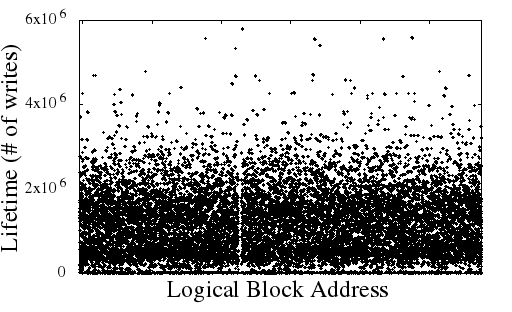
\includegraphics[width=0.215\textwidth]{figure/pcstream/lba_lifetime2}}  % data from 0/03031641
	\subfigure[Lifetime patterns over LBAs]{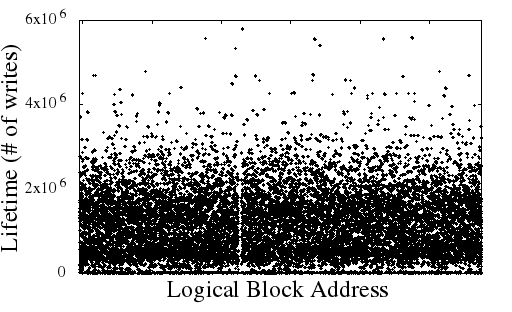
\includegraphics[scale=0.34]{figure/pcstream/lba_lifetime2}} \hspace{30pt}  % data from 0/03031641 
	\subfigure[Lifetime patterns over time]{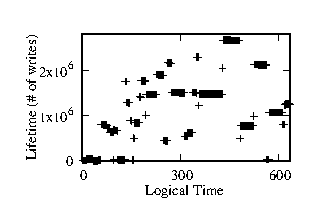
\includegraphics[scale=1]{figure/pcstream/lifetime_in_chunk}}
	%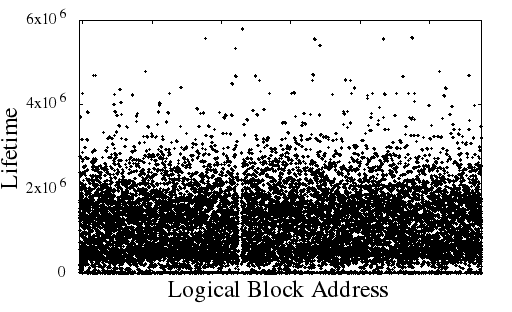
\includegraphics[width=0.9\linewidth]{figure/pcstream/lba_lifetime} 
	\caption{Lifetime distributions over addresses and times.} %shane part
	\label{fig:lba_lifetime}
\end{figure}


We also analyzed 
if the lifetimes of LBAs change under some predictable patterns over time 
although the overall lifetime distribution shows large variances.
Fig.~\ref{fig:lba_lifetime}(b) shows a scatter plot of data lifetimes over the logical time 
for a specific 1-MB chunk with 256 pages. 
As shown in Fig.~\ref{fig:lba_lifetime}(b), 
for the given chuck, data lifetimes vary in a random fashion
(although some temporal locality is observed).
\begin{comment}
Over the logical time, the lifetime of data written to the chunk 
varies in an unpredictable fashion.  
For example, at the logical time 10, the lifetime was 1 but it increases about 
2.6 million around the logical time 450 
followed by a rapid drop around the logical time 600. 
\end{comment}
Our illustration using RocksDB strongly suggests that under append-only
workloads, LBAs are not useful in deciding data lifetimes.

\subsection{Program context as a lifetime predictor}
In developing \textsf{\small PCStream}, our key insight was that in most applications,
%(regardless of their I/O workload characteristics)
a few dominant I/O activities exist
and each dominant I/O activity   
represents the application's important I/O context (e.g., for logging or for flushing). 
Furthermore, most dominant I/O activities tend to have distinct data lifetime patterns.
In order to distinguish data by their lifetimes, therefore, 
it is important to effectively distinguish dominant I/O activities from each other.  
For example, in update workloads, 
LBAs alone were effective in separating dominant I/O activities.  


\begin{comment}
In developing PCStream, we started from a simple question: 
how can we extract I/O context from an application? 
For example, in RocksDB, logging, flushing and compaction can be regarded
as different I/O contexts.
RocksDB appends write-ahead logs to storage to ensure data
persistence.  Those logs have short lifetimes because they are quickly deleted
after original data are persistently stored.
The flush module (which materializes the content of a memtable in
DRAM, called an L0 table, to an L1 table in the storage) generates data
with relatively short lifetimes. This is because an L1 table will be flushed to
an L2 table and be removed in the near future. Conversely, a compaction module
writes long-lived data that are unlikely to be removed for a long time.

The above observation implies that, if we are able to know the detailed
behaviors of append-only applications, data with different lifetimes can be
isolated in separate streams in an SSD. As mentioned before, a common
solution~\cite{MultiStream} to realizing this is manually modify an application
code so that each module assigns a unique stream ID to data it generates.
However, owing to considerable implementation efforts required to modify
individual applications, this approach is not widely used in practice.
\end{comment}

In this paper, we argue that a program context is an efficient  general-purpose
indicator for separating dominant I/O activities regardless of the type of I/O
workloads.  Since a PC represents an execution path of an application which
invokes write-related system functions such as {\tt write()} and {\tt writev()}
in the Linux kernel,  we represent the PC by summing program counter values of
all the functions along the execution path which leads to a write system call.
In RocksDB, for example, dominant I/O activities include logging, flushing and
compaction.  Since they are invoked through different function-call paths, we
can easily identify dominant I/O activities of RocksDB using PCs.  For example,
Fig.~\ref{fig:getpc}(a) shows an execution path for flushing in RocksDB.  The
sum of program counter values of \texttt{Run()}, \texttt{WriteLevel0Table()},
and \texttt{BuildTable()} is used to represent the PC for the flushing
activity.  Note that using the program context to distinguish data lifetimes is
not new.  For example, Ha {\it et al.} proposed a data separation technique
based on the program context~\cite{PCHa}.   However, their work was neither
designed for append-only workloads nor for modern multi-streamed SSDs.

\begin{figure}[t]
\centering
	\subfigure[Logging (PC)]{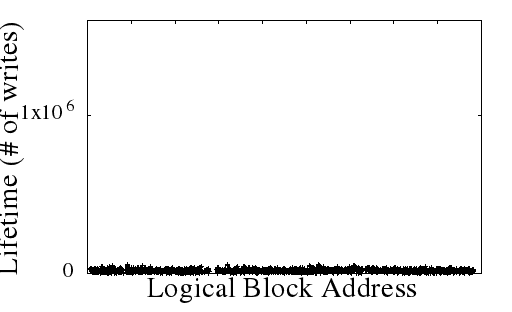
\includegraphics[scale=0.4]{figure/pcstream/type_1}} % data from 4/03031953 
	\hspace{10pt}
	\subfigure[Logging (manual)]{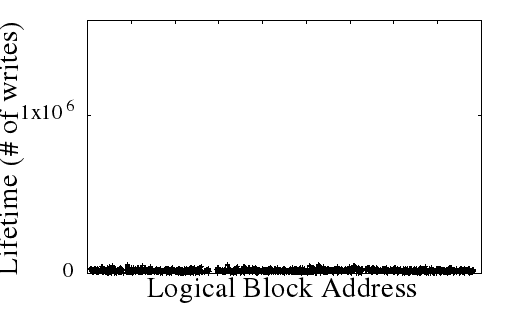
\includegraphics[scale=0.4]{figure/pcstream/pcID_2}}
	 \\
	\subfigure[Flushing (PC)] {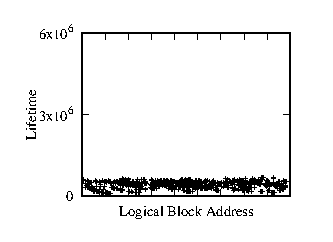
\includegraphics[scale=0.4]{figure/pcstream/type_3}}
	\hspace{10pt}
	\subfigure[Flushing (manual)]{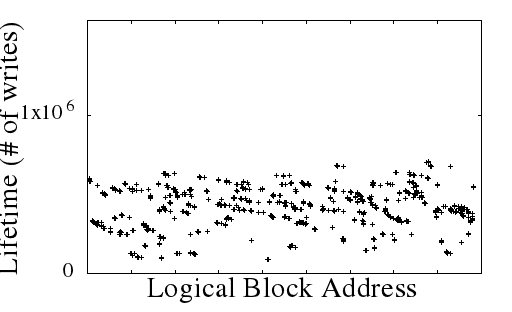
\includegraphics[scale=0.4]{figure/pcstream/pcID_3}}
\caption{Data lifetime distributions of different PCs.} 
\label{fig:types_and_PCs}
\end{figure}


In order to validate our hypothesis that PCs can be useful for predicting
lifetimes by distinguishing dominant I/O activities, we conducted experiments
using RocksDB, comparing the accuracy of identifying dominant I/O activities
using two different methods.  First, we manually identified dominant I/O
activities by inspecting the source code. Second, we automatically decided
dominant I/O activities by extracting PCs for write-related system functions.
Fig.~\ref{fig:types_and_PCs} illustrates two dominant I/O activities matched
between two methods.   As shown in Fig.~\ref{fig:types_and_PCs}(a)
and~\ref{fig:types_and_PCs}(b), the logging activity of RocksDB is correctly
identified by two methods.  Furthermore, from the logging-activity PC, we can
clearly observe that data written from the PC are short-lived. Similarly,
from Fig.~\ref{fig:types_and_PCs}(c) and~\ref{fig:types_and_PCs}(d), we observe
that data written from the flushing-activity PC behave in a different fashion.
For example, data from the flushing-activity PC remain valid a lot longer than
those from the logging-activity PC.

\section{Design of \textsf{PCStream}}
%We describe in detail the proposed automatic stream management technique, 
In this section, we describe in detail the proposed automatic stream management technique, %shane part
\textsf{\small PCStream}.  We first explain how we automatically extract PCs during
runtime and describe how multiple PCs are mapped to streams in an SSD.
In order to mitigate the side effect of a few outlier PCs with large lifetime variances, 
we introduce `substreams' based on a two-phase
stream assignment technique.
%{\it The PC extractor module}, which is implemented in the ... as part ... of a
%system call handler, computes a PC signature (i.e., a sum of program counter
%values) for each write-related system function. 추가 동작 설명..


Fig.~\ref{fig:architecture} shows an overall organization of \textsf{\small PCStream}.
\textit{The PC extractor module}, which is implemented in the Linux kernel as
part of a system call handler, 
computes a PC signature, which is used as a unique ID for each program context.  
We use the signature program counter~\cite{PC} as a PC signature 
by summing program counter values along the execution path to a write-related system function 
(e.g., {\tt write()}).  
With the PC signature, we can monitor the data lifetime of each write at the program context level. 
A PC signature value is stored
in an inode data structure of a file system (modified for \textsf{\small PCStream})
and is delivered to \textit{the lifetime analyzer module} which estimates
expected lifetimes of data belonging to a given PC in the block device level.
In order to efficiently detect the end of data lifetime in append-only
workloads, the lifetime analyzer also intercepts TRIM~\cite{TRIM} requests. %from a file system.  %shane part
Based on the lifetime information, \textit{the PC-to-stream
mapper module} clusters PCs with similar lifetimes and maps them together to
the same stream ID.  This mapping is required because 
the number of streams in an SSD is generally less than the number of PCs in host applications.

\subsection{Automatic PC computation}
As mentioned earlier, a PC is represented by a PC signature which is defined as
the sum of program counter values along the execution path of a function call that
%finally 
reaches a write-related system function. A function call involves
pushing the next program counter, which is used as a return address, to the
stack followed by pushing a frame pointer value.  In general, by using frame
pointer values, we are able to back-track the stack frames of the process and
selectively get return addresses for generating a PC signature.  For example,
Fig.~\ref{fig:getpc}(a) shows the abstracted execution path for flushing data
in RocksDB and Fig.~\ref{fig:getpc}(b) illustrates how a PC signature is obtained
by back-tracking the stack.  
Since a frame pointer value in the stack holds the address of the previous
%frame pointer, the PC extractor can easily obtain return addresses and
frame pointer, the PC extractor can obtain return addresses and
accumulate them to compute a PC signature. 
%(The return addresses are pushed
%before calling the \textsf{\small  write()}, \textsf{\small  BuildTable()} and \textsf{\small 
%WriteLevel0Table()} functions.)

\begin{figure}[t]
	\centering
	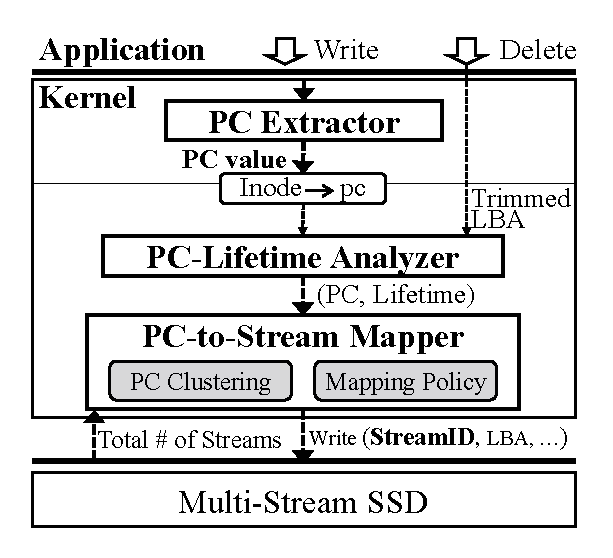
\includegraphics[width=0.6\linewidth]{figure/pcstream/architecture4}
	\caption{An overall architecture of \textsf{\small PCStream}.}
	\label{fig:architecture}
\end{figure}

%The PC extractor obtains and accumulates each
%return address, which is pushed before calling the \textsf{\small  write()}, \textsf{\small 
%BuildTable()} and \textsf{\small  WriteLevel0Table()} functions, by referring the frame
%pointer which holds the address of the previous frame pointer.

%Unfortunately, C/C++ compilers often optimize an output code so
%that it does not use a frame register if possible.  
The frame pointer-based approach for computing PC signatures, however, is not
always possible because modern C/C++ compilers often do not use the frame
pointer for improving the efficiency of register allocation.
One example is a
{\tt -fomit-frame-pointer} option of GCC~\cite{GCC}. 
%While it is effective in saving
%precious resources like CPU registers, this makes it difficult for us to
%back-track return addresses only. 
Although this option allows the frame pointer to be used as a general-purpose
register for high performance, it makes very difficult for us to back-track
return addresses along the call chains.  

\begin{figure}[t]
	\centering
	\subfigure[An abstracted execution path for flushing data.]{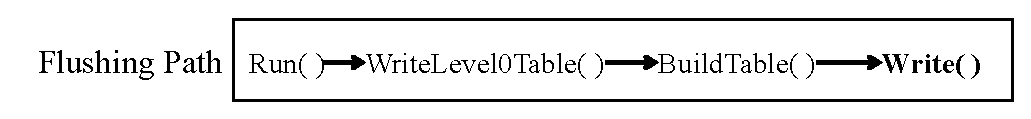
\includegraphics[scale=0.6]{figure/pcstream/getpc_1}}  
	\\
	\subfigure[with the frame pointer.]{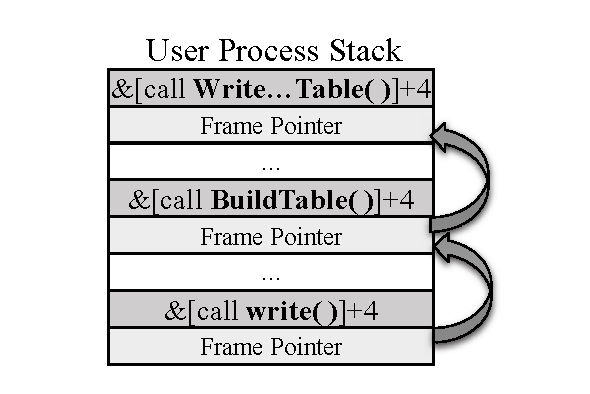
\includegraphics[scale=0.55]{figure/pcstream/getpc_2}}
	\hspace{10pt}
	\subfigure[without the frame pointer.]{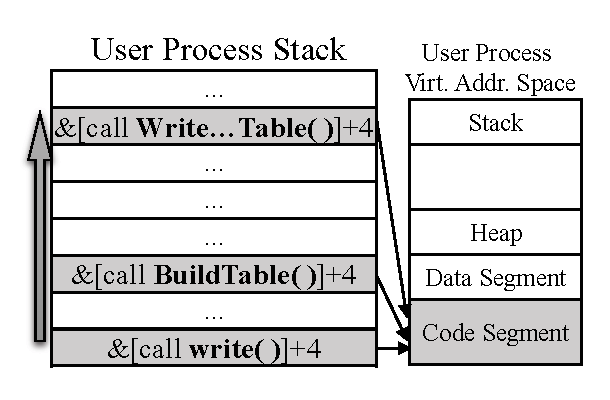
\includegraphics[scale=0.55]{figure/pcstream/getpc_3}}
	%\caption{An example execution path and its PC extraction methods.}
	\caption{An example execution path and its PC extraction.} %shane part
	\label{fig:getpc}
\end{figure}

In \textsf{\small PCStream}, we employ a simple but effective workaround 
for backtracking the call stack when the frame pointer is not used.
When a write system call is made, we scan every word in the stack and check
if it belongs to the process's code segment.  If the scanned stack word holds a
value within the address range of the code segment, we assume that it is a
return address.  Since scanning the full stack takes too long, we stop the
stack scanning procedure when a sufficient number of return address candidates
are found.  In the current version, we stop when 5 return address candidates
are found.  Although quite ad-hoc, a restricted scan is effective in
distinguishing different PCs because two different PCs
cannot follow the same execution path to write system functions.  
(If they do, they are the same PC.) In our evaluation
with a 3.4 GHz CPU machine, the performance overhead of the restricted scan was
almost negligible, taking only 300-400 $n$sec per write system call.

\subsection{PC lifetime prediction}

The prediction of PC lifetimes is rather complicated. 
The data lifetime of the append-only workload is defined 
from when a write request is issued until the TRIM command~\cite{TRIM} is issued to 
the corresponding address.
In order to measure the lifetime of data, the lifetime analyzer 
records the write time and PC value for each write request using its LBA.
Upon receiving the TRIM command, the lifetime analyzer can compute the 
lifetime of the corresponding data using the recorded information.
Note that, the
same PC may generate multiple data streams with different lifetimes.
We take the average lifetime as the PC's lifetime.

\subsection{Mapping PCs to SSD streams}

The last step in \textsf{\small PCStream} is to map
a group of PCs with similar lifetimes to an SSD stream.
This is because each SSD supports a limited number of stream IDs. For
example, SSDs used in \textsf{\small FStream}~\cite{FStream} and \textsf{\small AutoStream}~\cite{AutoStream}
support only 9 and 16 streams, respectively. To properly group multiple PCs,
the PC-to-stream mapper employs a simple 1-D clustering algorithm. 
In order to cluster PCs with similar lifetimes, the mapper calculates the 
lifetime difference between PCs.
Then, PCs with the smallest lifetime difference are clustered into the same PC group. 
The mapper repeats this clustering step until all the PCs are assigned to their PC groups.
For adapting to changing
workloads, reclustering operations should be regularly performed. Since the
number of PCs created by applications is not limited, the clustering algorithm
must be efficient enough to quickly handle many PCs. Our goal in this work is
to confirm the feasibility of using PCs, so we leave
those issues as our future work.

\subsection{Two-phase stream assignment}

For most PCs, their lifetime distributions tend to have small variances.  
However, we observed that a few outlier PCs which have large lifetime variations. 
For example, when multiple I/O contexts are covered by the same write system function, 
the corresponding PC may represent several I/O contexts whose data lifetimes are quite different.   
Such a case occurs %, for example, 
in the compaction module of RocksDB.
RocksDB maintains
several levels, L1, ..., L$n$, in the persistent storage, except for L0 (or a
memtable) stored in DRAM.  Once one level, say L2, becomes full, all the data
in L2 is compacted to a lower level, i.e., L3.  It involves moving data from L2
to L3, along with the deletion of the old data in L2.  In the
LSM tree~\cite{LSM}, a higher level is smaller than a lower level 
(i.e., the size of (L2) $<$ the size of (L3)). 
Thus, data stored in a higher level is invalidated more frequently than those kept
in lower levels, thereby having shorter lifetimes.

%Once the L1 becomes full,
%\textit{all} the data kept in the L1 are moved to the L2 by the compaction
%module.  The same operation is applied to the other levels (i.e., L3, ...,
%L$n-1$).  The compaction involves reading and writing data from a higher level
%(e.g., L1) to a lower level (e.g., L2).  The data in a higher level (e.g., L1)
%is then removed.  

%While the program context can be used as a useful indicator that determines the
%lifetime of data, we also observe that the same PC could generate data 
%with diverged lifetimes. One of the representative examples is the compaction
%module of RocksDB. RocksDB maintains several levels, L1, ..., L$n$, in the
%persistent storage, except for L0 (or a memtable) stored in DRAM.  Data flushed
%from the memtable are first written to the L1.  Once the L1 becomes full,
%\textit{all} the data kept in the L1 are moved to the L2 by the compaction
%module.  The same operation is applied to the other levels (i.e., L3, ...,
%L$n-1$).  The compaction involves reading and writing data from a higher level
%(e.g., L1) to a lower level (e.g., L2).  The data in a higher level (e.g., L1)
%is then removed.  In the LSM-tree, a higher level is smaller than a lower
%level. Thus, data stored in a higher level is invalidated sooner than data kept
%in lower levels, thereby having much shorter lifetimes.

Unfortunately, in the current RocksDB implementation, the compaction step is supported 
by the same execution path (i.e., the same PC) regardless of the level.
Therefore, the PC for the compaction activity cannot effectively separate data with 
short lifetimes from one with long lifetimes.
Fig.~\ref{fig:compaction}(a) shows 
the lifetime distribution collected from the compaction-activity PC.  
Since this distribution includes lifetimes of data written from all the levels, 
its variance is large.  
When we manually separate the single compaction step into several per-level compaction steps, 
as shown in Figs. 5(b) and 5(c), the lifetime distributions of per-level compaction steps 
show smaller variances.   
In particular, L2 and L3 show distinct lifetime distributions from that of L4.
Data from L2 and L3 are likely to have shorter lifetimes, while L4 has generally
long-lived data as shown in Fig. 5(d).

\begin{figure}[!t]
\centering
\subfigure[compaction: all levels]{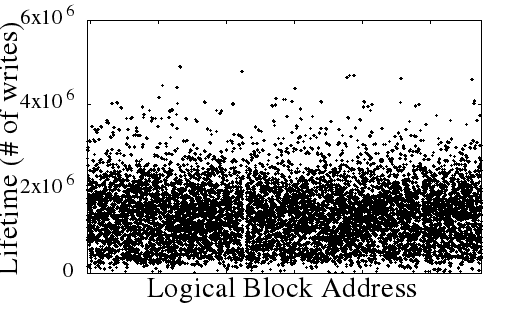
\includegraphics[scale=0.4]{figure/pcstream/pc_3}}
	\hspace{10pt}
\subfigure[compaction: L2]{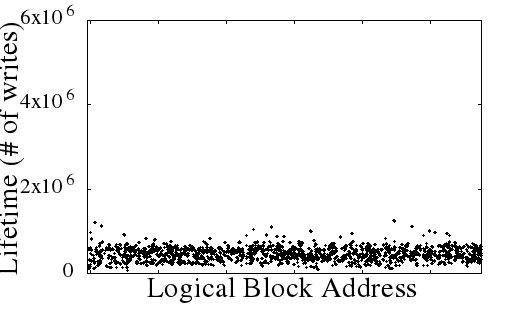
\includegraphics[scale=0.4]{figure/pcstream/type_4}}  % data from 4/03040047
\\
\subfigure[compaction: L3]{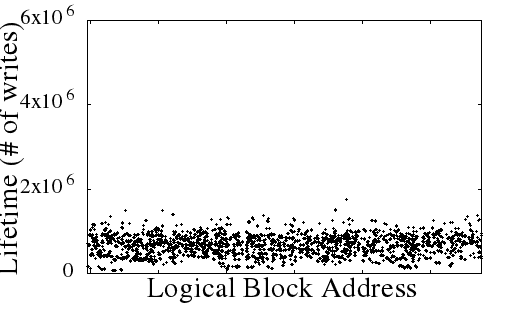
\includegraphics[scale=0.4]{figure/pcstream/type_5}}
	\hspace{10pt}
\subfigure[compaction: L4]{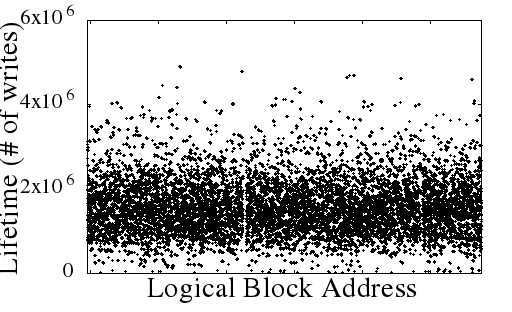
\includegraphics[scale=0.4]{figure/pcstream/type_6}}
%\caption{The lifetime distribution of the compaction activity.} 
\caption{Lifetime distributions of the compaction activity at different levels.} %shane part
\label{fig:compaction}
\end{figure}

Since it is difficult to separate data with different lifetimes within the same PC 
(as in the compaction-activity PC), we devised a two-phase method that decides SSD 
streams in two levels: the main stream ID in a host level and the substream ID in an SSD level.
Conceptually, long-lived data in the main stream are moved to its substream to 
separate from (future) short-lived data of the main stream.
Although moving data to the substream may increase WAF,
the overhead can be hidden if we restrict the substream move during GC only.
Since long-lived data (i.e., valid pages) in a victim block are moved to a free block during GC, 
they can be moved to the substream by changing the target block.
For instance, \textsf{\small PCStream} assigns the compaction-activity PC {\it pID} to a
main stream {\it sID} for the first phase.
To separate the long-lived data of {\it pID} (e.g., L4 data) 
from future short-lived data of {\it pID} (e.g., L1 data), 
valid pages of the {\it sID} are assigned to its substream for the second phase during GC.


\section{Experimental Results}

For our experiments, we have implemented \textsf{\small PCStream} in the Linux kernel
4.5.  For an objective evaluation, we compared \textsf{\small PCStream} with three
existing schemes: \textsf{\small Baseline}, \textsf{\small Manual}~\cite{MultiStream}, and
\textsf{\small AutoStream}~\cite{AutoStream}.  \textsf{\small Baseline} stands for a legacy
SSD that does not support a multi-stream feature. \textsf{\small Manual} is a RocksDB
implementation which is manually optimized for multi-streamed SSDs.
\textsf{\small AutoStream} is an LBA-based data separation technique which is
implemented at the device driver layer. To understand the impact of the
two-phase assignment, in addition, we compared \textsf{\small PCStream} with
\textsf{\small PCStream$^{*}$} which excluded the two-phase assignment feature.

For benchmarks, we have used three scenarios of \texttt{db\_bench} of RocksDB:
Update-Random (\texttt{UR}), Append-Random (\texttt{AR}), and Fill-Random
(\texttt{FR}) scenarios.  For key-value pairs already stored in the SSD,
\texttt{UR} updates values for random keys, creating many
read-modify-writes in the SSD.  \texttt{AR} is similar to \texttt{UR}, except
that it performs the update of values for growing keys. \texttt{FR} writes
key-value pairs to the SSD in a random key order.

\subsection{Experiments with an SSD emulator}

We carried out a set of experiments using an SSD emulator which is based on the
open flash development platform~\cite{AMF}.  
%The SSD emulator emulates the behaviors of an SSD using host DRAM in the kernel level. Thus, it not only allows us to easily add new features, but enables to analyze detailed internal activities of an SSD. 
In the SSD emulator, the internal workings of an SSD are simulated using the host's DRAM memory in the kernel level. 
For our evaluations, we extended the SSD emulator to support a multi-streamed feature %.
(up to 8 streams). %shane part
Furthermore, we enhanced the garbage collection module of the SSD firmware to support the two-phase stream management technique. 
%We assume that the SSD emulator supports up to 8 streams (as with Samsung PM963 which was used in our experiments). %shane part
%We enhanced the original emulator so that it supported a multi-streamed feature as well as the two-phase stream assignment.  The number of streams supported by the emulator was 8.  
The SSD emulator provided 12 GB capacity with 4 channels and 4 ways, and there were 8192 flash blocks, each of which was composed of 384 4-KB pages.  

\begin{figure*}[t]
	\centering
	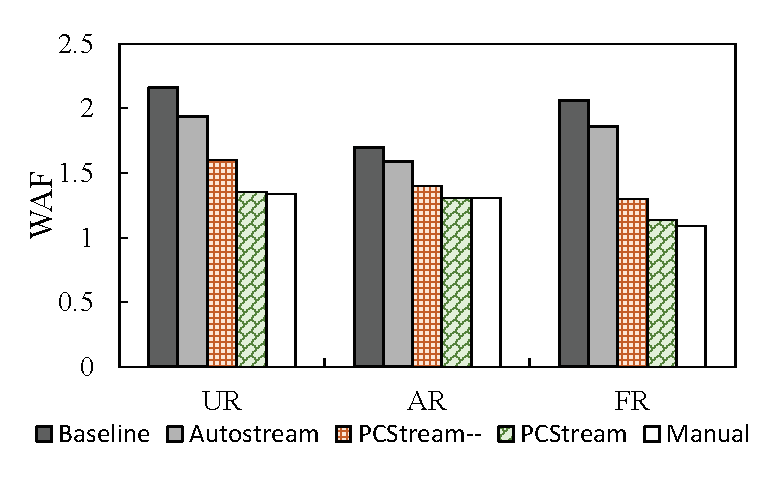
\includegraphics[scale=0.6]{figure/pcstream/result_emul}
	\caption{A comparison of WAF on the SSD emulator.}
	\label{fig:result_emul}
\end{figure*}


We compared WAF of the existing techniques with \textsf{\small PCStream} for the three
scenarios, and the result is shown in Fig.~\ref{fig:result_emul}.
\textsf{\small PCStream} was quite effective in reducing WAF, 
thus achieving an equivalent level of the WAF reduction as in \textsf{\small Manual}.  
For example, both \textsf{\small PCStream} and \textsf{\small Manual} reduced WAF by 38\% over \textsf{\small Baseline} for the \texttt{UR} case. 
%Compared with \textsf{\small AutoStream}, \textsf{\small PCStream} was more effective, reducing WAF more by 35\% on average.  
\textsf{\small PCStream} outperformed \textsf{\small AutoStream} by reducing WAF by 35\% on average.
Fig.~\ref{fig:result_emul} also indicates that the two-phase stream assignment technique is effective.  
\textsf{\small PCStream} outperformed \textsf{\small PCStream$^{*}$} by 12\% on average in the WAF reduction.
%As shown in Fig. 6, \textsf{\small PCStream$^*$} reduced WAF by up to 30\% over \textsf{\small AutoStream}.  
%The result shows that separating short-lived data (e.g., log and flush) from long-lived one (e.g., compaction) using PC was quite effective in reducing WAF.  Moreover, \textsf{\small PCStream} even showed similar WAF to \textsf{\small Manual}, reducing it by up to 38\% over \textsf{\small AutoStream}.  
This additional gain of \textsf{\small PCStream} over \textsf{\small PCStream$^{*}$} came from isolating long- and short-lived data in separate blocks 
%through the two-phase assignment at the SSD even if they belonged to the same compaction PC.
%by moving the long-lived data of the compaction-activity PC to substreams during GC at the SSD.
by moving the long-lived data to substreams during GC at the SSD.


In order to better understand how \textsf{\small PCStream} achieved a high reduction in WAF, 
we measured per-stream lifetime distributions under each technique for the \texttt{UR} scenario.
Fig.~\ref{fig:stream_lifetime} shows a box plot of data lifetimes from the 25th percentile to the 75th percentile.
%In order to analyze the improvement made by \textsf{\small PCStream}, 
%we measured the data lifetime of each stream for the {\tt UR} scenario.
%Fig. 7 shows average, 75p, and 25p of data liftime for each stream.

\begin{figure*}[t]
	\centering
	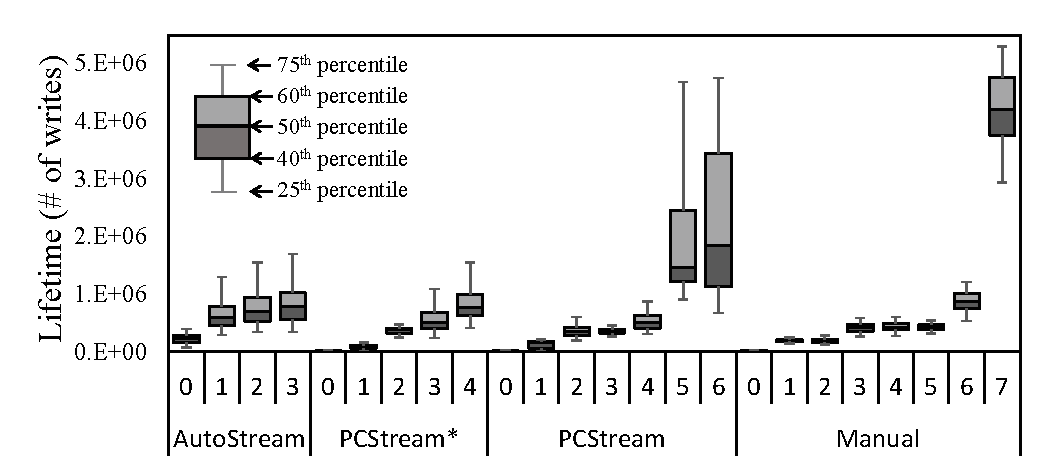
\includegraphics[scale=0.6]{figure/pcstream/stream_lifetime}
	\caption{A comparison of per-stream lifetime distributions.}
	\label{fig:stream_lifetime}
\end{figure*}



As shown in Fig.~\ref{fig:stream_lifetime}, 
streams in \textsf{\small PCStream} are divided into two groups, 
$G1$ = $\{$0, 1, 2, 3, 4$\}$ and $G2$ = $\{$5, 6$\}$, 
where $G1$ includes streams with short lifetimes and small variances %(i.e., streams 0, 1, 2, 3, and 4) 
and $G2$ includes streams with large lifetimes and large variances.  %(i.e., streams 5 and 6).  
%By preventing $G1$ and $G2$ from mixing in the same block, \textsf{\small PCStream} can reduce the GC overhead.  
Since the GC copy cost is affected by how data in $G1$ and $G2$ are mixed into the same block, 
\textsf{\small PCStream} can significantly reduce the GC overhead 
by avoiding such data mixtures in the same block by separating $G1$ and $G2$ into different streams. 
On the other hand, in \textsf{\small AutoStream}, 
three streams (i.e., streams 1, 2, and 3) show similar lifetime distributions with large variances 
without a distinct data separation pattern.
%Unlike \textsf{\small PCStream} and \textsf{\small Manual}, \textsf{\small AutoStream} does not show that 
%their streams are divided based on data lifetimes.  
%Such stream allocation is not effective in reducing the GC copy cost. 
%, thus not effectively taking full advantage of streams.
%data lifetimes of stream 0 to 5 in \textsf{\small Manual} are gathered in a narrow range so data lifetime in the same is quite similar.
%However, data lifetime of streams in \textsf{\small AutoStream} shows relatively large difference
%\textsf{\small AutoStream} does not notice when long-lived data is written to the hot stream.
%On the other hand, \textsf{\small PCStream$^*$} can identify short-lived data from 
%several dominant I/O activities as mentioned in section 2, for example, stream 0 and 1 in the Fig.~\ref{fig:stream_lifetime}.
%\textsf{\small PCStream} can further separate long-lived data of several streams (e.g., stream 3 and 4)
%by moving their data to substreams (e.g., stream 5 and 6, respectively). 
In Fig.~\ref{fig:stream_lifetime}, we can also observe the effect of substreams.  
Streams 3 and 4 of \textsf{\small PCStream$^{*}$}, 
which have large variances in lifetimes, are split into two substreams 5 and 6 in \textsf{\small PCStream}.
This split reduces variances of streams 3 and 4, thus reducing the GC copy cost.  %improving WAF. 

\subsection{Experiments with a real-world SSD}

In order to evaluate the effect of \textsf{\small PCStream} in a real SSD,  
%In order to confirm the feasibility of \textsf{\small PCStream}, 
we have
conducted experiments using Samsung's PM963 480GB SSD that supports 8 streams.
Since it was impossible to implement the two-phase stream assignment in the
commercial SSD firmware, we evaluated \textsf{\small PCStream$^*$} only.  To warm up the
SSD before running benchmarks, we filled up 90\% of the SSD capacity with valid
data.

\begin{figure*}[t]
	\centering
	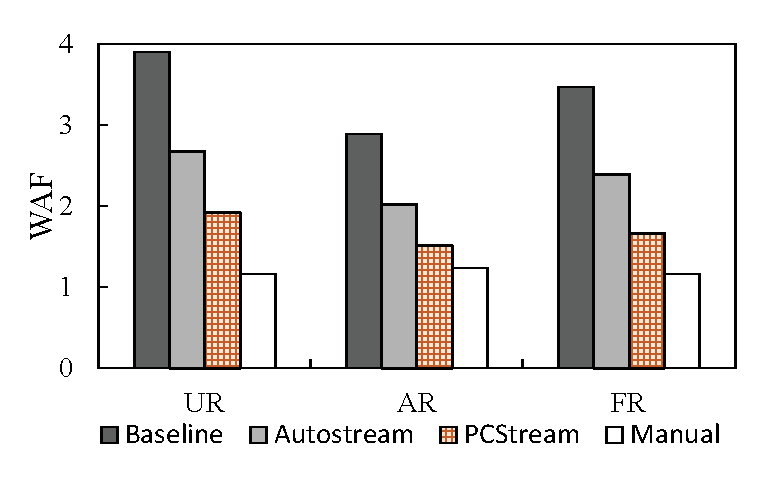
\includegraphics[scale=0.6]{figure/pcstream/result_ssd}
	\caption{A comparison of WAF on Samsung PM963 SSD.}
	\label{fig:result_ssd}
\end{figure*}


As illustrated in Fig.~\ref{fig:result_ssd}, \textsf{\small PCStream$^*$} reduced WAF by
28\% over \textsf{\small AutoStream} on average.  
%There were large WAF gaps between \textsf{\small PCStream$^{*}$} and the manually optimized case.  If the substream was properly supported during GC, we believe that \textsf{\small PCStream} could show similar WAF values as \textsf{\small Manual}.  
Note that although \textsf{\small PCStream$^*$} still outperformed \textsf{\small AutoStream} in PM963, 
but a performance gap was smaller over that
in the emulated SSD environment.  It was difficult to pinpoint why
\textsf{\small AutoStream} worked better in PM963 over in the emulated SSD, but we
suspect that some internal features of PM963 (such as a large block size or some implementation details of streams) %might be related. 
might have affected the performance of \textsf{\small AutoStream}.


\section{Conclusions}

We have presented a new stream management technique, \textsf{\small PCStream}, for multi-streamed SSDs.  
Unlike existing stream management techniques, \textsf{\small PCStream} fully automates 
the process of mapping data to a stream based on PCs, 
which work well for append-only workloads as well as update workloads.  
By exploiting an observation that most PCs are distinguishable from each other 
in their lifetime characteristics, \textsf{\small PCStream} allocates each PC to a different stream.  
When a PC has a large variance in their lifetimes, \textsf{\small PCStream} refines its stream allocation 
during garbage collection and moves the long-lived data of the current stream to its substream.  
%Our experimental results show that \textsf{\small PCStream} can reduce WAF by up to 38\% over the existing
Our experimental results show that \textsf{\small PCStream} can reduce the average WAF by 35\% over the existing %shane part
automatic technique.

The current version of \textsf{\small PCStream} can be extended in several directions.  
For example, we plan to optimize the PC clustering method so that
multiple PCs can be better clustered when the number of PCs significantly
outnumbers the number of streams.  
%For example, \textsf{\small PCStream} should be improved in its PC clustering method 
%so that it can work effectively even when there are more PCs than the number of streams.  
%We also plan to evaluate \textsf{\small PCStream} (not \textsf{\small PCStream}$^{--}$) on real SSDs 
%by implementing the two-phase stream assignment algorithm inside an FTL.

\chapter{FineDedup} 
\label{chap:FineDedup}



\chapter{Conclusions}
\label{chap:Conclusions}

\section{Summary and Conclusions}


The cost-per-bit of NAND flash-based solid-state drives (i.e., SSDs) has steadily improved through uninterrupted semiconductor process scaling and multi-leveling so that they are how widely employed in not only mobile embedded systems but also personal computing systems.
However, the limited lifetime of NAND flash memory, as a side effect of recent advanced device technologies, is emerging as one of the major concerns for recent high-performance SSDs, especially for datacenter applications.




%\clearpagebefore
%\phantomsection
%\addcontentsline{toc}{chapter}{Bibliography}
%\begin{onehalfspacing}
%\bibliographystyle{ieeetr}
%\bibliography{ref}
%\bibliography{reference}
%\end{onehalfspacing}

%\begin{thebibliography}{00}
%\end{thebibliography}

\begin{thebibliography}{00}
\addcontentsline{toc}{chapter}{\bibname}

% 영문저널의 경우
%    \bibitem{ref1} B. Jeon and J. Jeong, ``Blocking artifacts
%    reduction in image compression with block boundary discontiunity
%    criterion,'' {\em IEEE Transactions on Circuits and Systems for
%    Video Tech.}, vol. 8, no.3, pp. 345-357, June 1998.

% 영문학술대회의 경우
%    \bibitem{ref2} W. G. Jeon and Y. S. Cho, ``An equalization
%    technique for OFDM and MC-CDMA in a multipath fading channels,''
%    in {\em Proceedings of IEEE Conference on Acoustics, Speech and
%    Signal Processing}, Munich, Germany, May 1997. pp. 2529-2532.

% 단행본의 경우
%    \bibitem{ref4} C. Mead and L. Conway, {\em Introduction to VLSI
%    Systems}, Addison-Wesley, Boston, 1994.

% URL
%    \bibitem{ref5} The SolarMESH Network,
%    http://owl.mcmater.ca/solarmesh

% Technical Report의 경우
%    \bibitem{ref6} K. E. Elliott and C. M. Greene, ``A local adaptive
%    protocol,'' Argonne National Laboratory, Argonne, France,
%    Technical Report 916-1010-BB, 1997.

% 학위논문의 경우
%    \bibitem{ref7} T. Kim, ``Scheduling and Allocation Problems in
%    High-level Synthesis,'' Ph. D. Dissertation, ECE Department,
%    Univ. of Illinois at U-C, 1993.

% 특허의 경우
%    \bibitem{ref8} Sunghyun Choi, ``Wireless MAC protocol based on a
%    hybrid combination of slot allocation, token passing, and
%    polling for isochronous traffic,'' U.S. Patent No. 6,795,418,
%    September 21, 2004.

% 표준
%    \bibitem{ref9} IEEE Std. 802.11-1999, Part 11: Wireless LAN
%    Medium Access Control (MAC) and Physical Layer (PHY)
%    specifications, Reference number ISO/IEC 8802-11:1999(E), IEEE
%    Std. 802.11, 1999 edition, 1999.


\bibitem{Janus_albrecht}
C.~Albrecht, A.~Merchant, M.~Stokely, M.~Waliji, F.~Labelle, N.~Coehlo, X.~Shi, and C.~E.~Schrock,
``Janus: Optimal Flash Provisioning for Cloud Storage Workloads,"
in \emph{Proceedings of the USENIX Annual Technical Conference} (ATC), 2013.

\bibitem{15nmMLC_Sako}
Mario Sako
Y.~Watanabe, T.~Nakajima, J.~Sato, K.~Muraoka, M.~Fujiu, F.~Kouno, M.~Nakagawa, M.~Masuda, K.~Kato, Y.~Terada, Y.~Shimizu, M.~Honma, A.~Imamoto,  T.~Araya, H.~Konno, T.~Okanaga, T.~Fujimura, X.~Wang, M.~Muramoto, M.~Kamoshida, M.~Kohno, Y.~Suzuki, T.~Hashiguchi, T.~Kobayashi, M.~Yamaoka, and R.~Yamashita,
``A Low-Power 64Gb MLC NAND-Flash Memory in 15 nm CMOS Technology,"
in \emph{Proceedings of the IEEE International Solid-State Circuits Conference} (ISSCC), 2015.

\bibitem{21nmMLC_Kim}
C.~Kim, J.~Ryu, T.~Lee, H.~Kim, J.~Lim, J.~Jeong, S.~Seo, H.~Jeon, B.~Kim, I.~Lee, D.~Lee, P.~Kwak, S.~Cho, Y.~Yim, C.~Cho, W.~Jeong, K.~Park, J.-M.~Han, D.~Song, K.~Kyung, Y.-H.~Lim, and Y.-H.~Jun,
``A 21 nm High Performance 64 Gb MLC NAND Flash Memory with 400 MB/s Asynchronous Toggle DDR Interface,"
\emph{IEEE Journal of Solid-State Circuits}, vol. 47, no. 4, pp. 981--989, 2012.

\bibitem{TLC_Shin}
S.-H.~Shin, D.-K.~Shim, J.-Y.~Jeong, O.-S.~Kwon, S.-Y.~Yoon, M.-H.~Choi, T.-Y.~Kim, H.-W.~Park, H.-J.~Yoon, Y.-S.~Song, Y.-H.~Choi, S.-W.~Shim, Y.-L.~Ahn, K.-T.~Park, J.-M.~Han, K.-H.~Kyung, and Y.-H.~Jun,
``A New 3-bit Programming Algorithm using SLC-to-TLC Migration for 8 MB/s High Performance TLC NAND Flash Memory,"
in \emph{the IEEE Symposium on VLSI Circuits Digest of Technical Papers} (VLSI), 2012.

\bibitem{Flash_Brewer}
J.~E.~Brewer and M.~Gill,
``Nonvolatile Memory Technologies with Emphasis on Flash,"
\emph{Wiley}, 2008.

\bibitem{MooresLaw_chien}
A.~A.~Chien and V.~Karamcheti,
``Moore's Law: The First Ending and a New Beginning,"
\emph{IEEE Computer Magazine}, vol. 46, no. 12, pp. 48--53, 2013.

\bibitem{HotCold_Hsieh}
J.-W. Hsieh, T.-W.~Kuo, and L.-P.~Chang,
``Efficient Identification of Hot Data for Flash Memory Storage Systems,"
\textit{ACM Transactions on Storage}, vol. 2, no. 1, pp. 22--40, 2006.

\bibitem{CAFTL_Chen}
F.~Chen, T.~Luo, and X.~Zhang,
``CAFTL: A Content-Aware Flash Translation Layer Enhancing the Lifespan of Flash Memory Based Solid State Drives,"
in \textit{Proceedings of the USENIX Conference on File and Storage Technologies} (FAST), 2011.

\bibitem{Compression_Lee}
S.~Lee, J.~Park, K.~Fleming, Arvind, and J.~Kim,
``Improving Performance and Lifetime of Solid-State Drives Using Hardware-Accelerated Compression,"
\textit{IEEE Transactions on Consumer Electronics}, vol. 57, no. 4, pp. 1732--1739, 2011.

\bibitem{DT_Lee}
S.~Lee, T.~Kim, K.~Kim, and J.~Kim,
``Lifetime Management of Flash-Based SSDs Using Recovery-Aware Dynamic Throttling,"
in \textit{Proceedings of the USENIX Conference on File and Storage Technologies} (FAST), 2012.

\bibitem{SelfHealing_Wu}
Q.~Wu, G.~Dong, and T.~Zhang,
``Exploiting Heat-Accelerated Flash Memory Wear-Out Recovery to Enable Self-Healing SSDs,"
in \emph{Proceedings of the USENIX Workshop on Hot Topics in Storage and File Systems} (HotStorage), 2011.

\bibitem{RetentionRelaxation_Liu}
R.-S.~Liu, C.-L.~Yang, and W.~Wu,
``Optimizing NAND Flash-Based SSDs via Retention Relaxation,"
in \textit{Proceedings of the USENIX Conference on File and Storage Technologies} (FAST), 2012.

\bibitem{Flexfs_Lee}
S.~Lee, K.~Ha, K.~Zhang, J.~Kim, and J.~Kim,
``FlexFS: A Flexible Flash File System for MLC NAND Flash Memory,"
in \emph{Proceedings of the USENIX Annual Technical Conference} (ATC), 2009.

\bibitem{Cox_JEDEC}
A.~Cox,
``JEDEC SSD Specifications Explained,"
Available: http://www.jedec.org.

\bibitem{DPES_jeong}
J.~Jeong, S.~S.~Hahn, S.~Lee, and J.~Kim,
``Lifetime Improvement of NAND Flash-based Storage Systems Using Dynamic Program and Erase Scaling," 
in \emph{Proceedings of the USENIX Conference on File and Storage Technologies} (FAST), 2014.

\bibitem{BER_mielke}
N.~Mielke, T.~Marquart, N.~Wu, J.~Kessenich, H.~Belgal, E.~Schares, F.~Trivedi, E.~Goodness, and L.~R.~Nevill,
``Bit Error Rate in NAND Flash Memories,"
in \emph{Proceedings of the International Reliability Physics Symposium} (IRPS), 2008.

\bibitem{ReadDisturb_Kang}
M.~Kang, K.-T.~Park, Y.~Song, S.~Hwang, B.~Y.~Choi, Y.~Song, Y.~Lee, and C.~Kim,
``Improving Read Disturb Characteristics by Self-Boosting Read Scheme for Multilevel NAND Flash Memories,"
\emph{Japanese Journal of Applied Physics}, vol. 48, no. 4, pp. 04C062-1--04C062-6, 2009.

\bibitem{ISPP_suh}
K.-D.~Suh, B.-H.~Suh, Y.-H.~Lim, J.-K.~Kim, Y.-J.~Choi, Y.-N.~Koh, S.-S.~Lee, S.-C.~Kwon, B.-S.~Choi, J.-S.~Yum, J.-H.~Choi, J.-R.~Kim, and H.-K.~Lim,
``A 3.3 V 32 Mb NAND Flash Memory with Incremental Step Pulse Programing Scheme,"
\emph{IEEE Journal of Solid-State Circuits}, vol. 30, no. 11, pp. 1149--1156, 1995.

\bibitem{FN_schuegraf}
K.~F.~Schuegraf and C.~Hu,
``Effects of Temperature and Defects on Breakdown Lifetime of Thin SiO2 at Very Low Voltages,"
\emph{IEEE Transactions on Electron Devices}, vol. 41, no. 7, pp. 1227--1232, 1994.

\bibitem{TR_jeong}
J.~Jeong and J.~Kim,
``Dynamic Program and Erase Scaling in NAND Flash-based Storage Systems,"
\emph{Technical Report, Seoul National University},
cares.snu.ac.kr/download/TR-CARES-01-14, 2014.

\bibitem{Reliability_cho}
S.~Cho,
``Improving NAND Flash Memory Reliability with SSD Controllers,"
in \emph{Proceedings of the Flash Memory Summit}, 2013.

\bibitem{JEDEC}
JEDEC standard,
``Stress-Test-Driven Qualification of Integrated Circuits,"
JESD47H.01, 2011.

\bibitem{ISPE_Lee}
D.~W.~Lee, S.~Cho, B.~W.~Kang, S.~Park, B.~Park, M.~K.~Cho, K.-O.~Ahn, Y.~S.~Yang, and S.~W.~Park,
``The Operation Algorithm for Improving the Reliability of TLC (Triple Level Cell) NAND Flash Characteristics,"
in \emph{Proceedings of the IEEE International Memory Workshop} (IMW), 2011.

\bibitem{Flashbench_lee}
S.~Lee, J.~Park, and J.~Kim,
``FlashBench: A Workbench for a Rapid Development of Flash-based Storage Devices,"
in \emph{Proceedings of the IEEE International Symposium on Rapid System Prototyping} (RSP), 2012.

\bibitem{Revisiting_Jung}
M.~Jung and M.~Kandermir,
``Revisiting Widely Held SSD Expectations and Rethinking System-Level Implications,"
in \emph{Proceedings of the ACM SIGMETRICS}, 2013.

\bibitem{WL_Chang}
L.-P. Chang,
``On Efficient Wear Leveling for Large-Scale Flash-Memory Storage Systems,"
in \textit{Proceedings of the ACM Symposium on Applied Computing}, 2007.

\bibitem{ReadRetry_Yang}
J. Yang,
``High-Efficiency SSD for Reliable Data Storage Systems,"
in \textit{Proceedings of the Flash Memory Summit}, 2011.

\bibitem{Reliability_Frickey}
R. Frickey,
``Data Integrity on 20 nm NAND SSDs,"
in \textit{Proceedings of the Flash Memory Summit}, 2012.

\bibitem{Hrtimer}
IBM,
``Kernel APIs, Part 3: Timers and Lists in the 2.6 Kernel,"
http://www.ibm.com/developerworks/library/l-timers-list/.

\bibitem{Narayanan2008}
D. Narayanan, A.~Donnelly, and A.~Rowstron,
``Write Off-Loading: Practical Power Management for Enterprise Storage,"
in \textit{Proceedings of the USENIX Conference on File and Storage Technologies} (FAST), 2008.

\bibitem{Ubuntu}
http://www.ubuntu.com/download

\bibitem{PreemptionGC_Lee}
J.~Lee, Y.~Kim, G.~M.~Shipman, S.~Oral, and J.~Kim,
``Preemptible I/O Scheduling of Garbage Collection for Solid State Drives,"
\emph{IEEE Transactions on Computer-Aided Design of Integrated Circuits and Systems}, vol. 32, no. 2, pp. 247--260, 2013.

\bibitem{PowerHoldUp_Bang}
K.~Bang, K.-I.~Im, D.-G.~Kim, S.-H.~Park, and E.-Y.~Chung,
``Power Failure Protection Scheme for Reliable High-Performance Solid State Disks,"
\emph{IEICE Transactions on Information and Systems}, vol. E96-D, no. 5, pp. 1078--1085, 2013.

\bibitem{Trimming_shi}
L.~Shi, K.~Wu, M.~Zhao, C.~J.~Xue, and E.~H.-M. Sha,
``Retention Trimming for Wear Reduction of Flash Memory Storage Systems,"
in \emph{Proceedings of the Design Automation Conference} (DAC), 2014.

\bibitem{JEDEC_Arrenius}
JEDEC standard,
``Method for Developing Acceleration Models for Electronic Component Failure Mechanisms,"
\emph{JESD91A}, Aug. 2003.

\bibitem{Yu_RFR}
Y.~Cai, Y.~Luo, E.~F.~Haratsch, K.~Mai, and O.~Mutlu,
``Data Retention in MLC NAND Flash Memory: Characterization, Optimization, and Recovery,"
in \emph{Proceedings of the IEEE Symposium on High-Performance Computing Architecture} (HPCA), 2015.

\bibitem{Takeuchi_DRRP}
S.~Tanakamaru, Y.~Yanagihara, and K.~Takeuchi,
``Error-Prediction LDPC and Error-Recovery Schemes for Highly Reliable Solid-State Drives (SSDs),"
\emph{IEEE Journal of Solid-State Circuits}, vol. 48, no. 11, pp. 2920--2933, 2013.

\bibitem{FD_Jeong}
J.~Jeong, Y.~Song, and J.~Kim,
``FlashDefibrillator: A Data Recovery Technique for Retention Failures in NAND Flash Memory,"
in \emph{Proceedings of the IEEE Non-Volatile Memory System and Applications Symposium} (NVMSA), 2015.

\bibitem{Fukuda_RTN}
K.~Fukuda, Y.~Shimizu, K.~Amemiya, M.~Kamoshida, and C.~Hu,
``Random Telegraph Noise in Flash Memories - Model and Technology Scaling,"
in \emph{Proceedings of the IEEE International Electron Devices Meeting} (IEDM), 2007.

\bibitem{Tang_ReadDisturbance}
B.~Tang, C.~Robinson, W.~D.~Zhang, J.~F.~Zhang, R.~Degraeve, P.~Blomme, M.~Toledano-Luque, G.~V.~den bosch, B.~Govoreanu, and J.~V.~Houdt,
``Read and Pass Disturbance in the Programmed States of Floating Gate Flash Memory Cells With High-$k$ Interpoly Gate Dielectric Stacks,"
\emph{IEEE Transactions on Electron Devices}, vol. 60, no. 7, pp. 2261--2267, 2013.

%\bibitem{Refresh_Cai}
%Y.~Cai, G.~Yalcin, O.~Mutlu, E.~F.~Haratsch, A.~Cristal, O.~S.~Unsal, and K.~Mai,
%``Flash Correct-and-Refresh: Retention-Aware Error Management for Increased Flash Memory Lifetime,"
%in \emph{Proceedings of the IEEE International Conference on Computer Design} (ICCD), 2012.

\bibitem{ReadDisturb_Ha}
K.~Ha, J.~Jeong, and J.~Kim,
``An Integrated Approach for Managing Read Disturbs in High-Density NAND Flash Memory,"
accepted for publication in \emph{IEEE Transactions on Computer-Aided Design of Integrated Circuits and Systems}.

\bibitem{SSDAlloc_Badam}
A.~Badam and V. S. Pai,
``SSDAlloc: Hybrid SSD/RAM Memory Management Made Easy,"
in \emph{Proceedings of the USENIX Conference on Networked Systems} (NSDI), 2011.

\bibitem{FlashMainMemory_Jacob}
B.~Jacob, I.~Bhati, M.-T.~Chang, P.~Rosenfeld, J.~Stevens, P.~Tschirhart, Z.~Chishti, S.-L.~Lu, J.~Ang, D.~Resnick, and A.~Rodrigues,
``A Journaled, NAND-Flash Main-Memory System,"
\emph{Technical Report, University of Maryland}, UMD-SCA-2010-12-01, December 2010, updated 2014.

\bibitem{Flash_Facebook}
J.~Taylor,
``Flash at Facebook,"
in \emph{Proceedings of the Flash Memory Summit}, 2013.

\end{thebibliography}

%\input{abstract_ko.tex}

%========================================================================
% index 
\clearpagebefore
\phantomsection
\addcontentsline{toc}{chapter}{Appendix}
\printindex

%========================================================================
% thanksto
%\input{thanks.tex}

\normalsize
\end{document}
